\documentclass[12pt]{article}
\usepackage{amssymb, enumerate, amsmath, amsthm}
\usepackage{graphics}
\usepackage{pgfplots}
\usepackage{txfonts}

\newcommand{\problem}[1]{\bigskip \noindent \textbf{Problem #1}}
\newcommand{\Call}{\text{Call}}
\newcommand{\Put}{\text{Put}}
\newcommand{\PV}{\text{PV}}
\newcommand{\Straddle}{\text{Straddle}}

\theoremstyle{plain}
\newtheorem{theorem}{Theorem}[section]
\newtheorem{corollary}[theorem]{Corollary}
\newtheorem{lemma}[theorem]{Lemma}
\newtheorem{proposition}[theorem]{Proposition}
\newtheorem{conjecture}[theorem]{Conjecture}
\newtheorem{question}{Question}
\newtheorem*{theorem*}{Theorem}
\newtheorem*{example*}{Example}
\newtheorem*{definition*}{Definition}
\newtheorem*{nonexample*}{Non-Example}


\setlength{\oddsidemargin}{0in}
\setlength{\textwidth}{6.5in}
\setlength{\topmargin}{0in}
\setlength{\headheight}{0in}
\setlength{\headsep}{0in}
\setlength{\textheight}{8.7in}
\title{McDonald Exercises, Chapter 3}
\author{Christophe Dethier}
\date{$\substack{\text{Created September 2, 2020}\\\text{Last edited \today}}$}
\begin{document}
\bigskip
\maketitle

Please contact me at christophehldethier@gmail.com with any questions, comments, or corrections.

\problem{3.1} Suppose that you buy the S\&R index for \$1000, buy a 1000-strike put, and borrow \$980.39. Perform a payoff and profit calculation mimicking table 3.1. Graph the resulting payoff and profit diagrams for the combined position.\\

For this problem I'm assuming that the effective 6-month interest rate on the loan is also 2\%.

The table below lists payoffs and profits for this position depending on various values of the S\&R index after 6 months:

\begin{center}
Long Index, Loan, and Purchased Put
\begin{tabular}{l||ccccccc}
S\&R Index (\$) & 900 & 950 & 1000 & 1050 & 1100 & 1150 & 1200 \\ \hline \hline
S\&R Put (\$) & 100 & 50 & 0 & 0 & 0 & 0 & 0 \\
Loan (\$) & -1000 & -1000 & -1000 & -1000 & -1000 & -1000 & -1000 \\
Payoff (\$) & 0 & 0 & 0 & 50 & 100 & 150 & 200 \\
-(Cost + Interest) (\$) & -95.68 & -95.68 & -95.68 & -95.68 & -95.68 & -95.68 & -95.68 \\
Profit (\$) & -95.68 & -95.68 & -95.68 & -45.68 & 4.32 & 54.32 & 104.32
\end{tabular}.
\end{center}
The payoff and profit diagrams for this position are graphed below:

\begin{center}
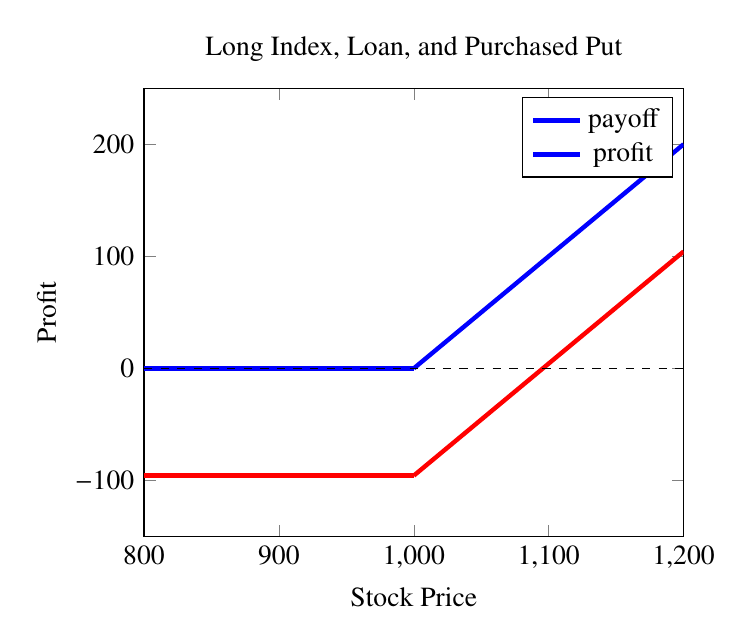
\begin{tikzpicture}
\begin{axis}[
disabledatascaling,
anchor=origin,
xmin=800,xmax=1200,
ymin=-150,ymax=250, 
xlabel=Stock Price,
ylabel=Profit,
title=\text{Long Index, Loan, and Purchased Put},
samples=50]
  \addplot[blue, ultra thick, domain=800:1000] (x,0);
  \addplot[blue, ultra thick, domain=1000:1200] (x,x-1000);
  \addlegendentry{payoff};
  \addplot[red, ultra thick, domain=800:1000] (x,0-95.68);
  \addplot[red, ultra thick, domain=1000:1200] (x,x-1000-95.68);
  \addlegendentry{profit};
  \addplot[black, dashed, domain=800:1200] (x,0);
\end{axis}
\end{tikzpicture}
\end{center}

\problem{3.2} Suppose that you short the S\&R index for \$1000 and sell a 1000-strike put. Construct a table mimicking Table 3.1 that summarizes the payoff and profit of this position. Verify that your table matches Figure 3.5.\\

The table below lists payoffs and profits for this position depending on various values of the S\&R index after 6 months. Note that the initial revenue of \$1000 from shorting the stock increases in value to \$1020 due to the 2\% effective 6-month interest rate.

\begin{center}
Short Index and Written 1000-Strike Put
\begin{tabular}{l||ccccccc}
S\&R Index (\$) & 900 & 950 & 1000 & 1050 & 1100 & 1150 & 1200 \\ \hline \hline
Short (\$) & 100 & 50 & 0 & -50 & -100 & -150 & -200 \\
Put (\$) & -100 & -50 & 0 & 0 & 0 & 0 & 0 \\
Payoff (\$) & 0 & 0 & 0 & -50 & -100 & -150 & -200 \\
Premium + Interest (\$) & 95.68 & 95.68 & 95.68 & 95.68 & 95.68 & 95.68 & 95.68 \\
Profit (\$) & 95.68 & 95.68 & 95.68 & 45.68 & -4.32 & -54.32 & -104.32
\end{tabular}.
\end{center}
To verify that this matches Figure 3.5, the payoff and profit diagrams are drawn below:
\begin{center}
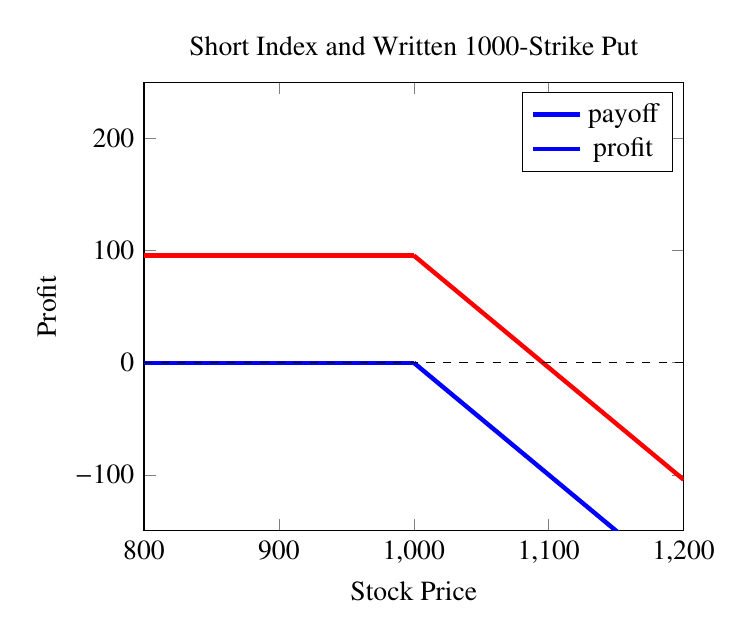
\begin{tikzpicture}
\begin{axis}[
disabledatascaling,
anchor=origin,
xmin=800,xmax=1200,
ymin=-150,ymax=250, 
xlabel=Stock Price,
ylabel=Profit,
title=\text{Short Index and Written 1000-Strike Put},
samples=50]
  \addplot[blue, ultra thick, domain=800:1000] (x,0);
  \addplot[blue, ultra thick, domain=1000:1200] (x,1000-x);
  \addlegendentry{payoff};
  \addplot[red, ultra thick, domain=800:1000] (x,95.68);
  \addplot[red, ultra thick, domain=1000:1200] (x,-x+1000+95.68);
  \addlegendentry{profit};
  \addplot[black, dashed, domain=800:1200] (x,0);
\end{axis}
\end{tikzpicture}
\end{center}

\bigskip
For the following problems assume the effective 6-month interest rate is 2\%, the S\&R 6-month forward price is \$1020, and use these premiums for S\&R options with 6 months to expiration:
\begin{center}
\begin{tabular}{l||ccccc}
\textbf{Strike (\$)} & 950 & 1000 & 1020 & 1050 & 1107 \\
\textbf{Call (\$)} & 120.405 & 93.809 & 84.470 & 71.820 & 51.873\\
\textbf{Put (\$)} & 51.777 & 74.201 & 84.470 & 101.214 & 137.167
\end{tabular}.
\end{center}

\problem{3.3} Suppose you buy the S\&R index for \$1000 and buy a 950-strike put. Construct payoff and profit diagrams for this position. Verify that you obtain the same payoff and profit diagram by investing \$931.37 in zero-coupon bonds and buying a 950-strike call.\\

First we calculate the future value of the cost of the put to be \$52.813, and the future of the investment to be \$1020. Here is the payoff and profit diagram for this position:

\begin{center}
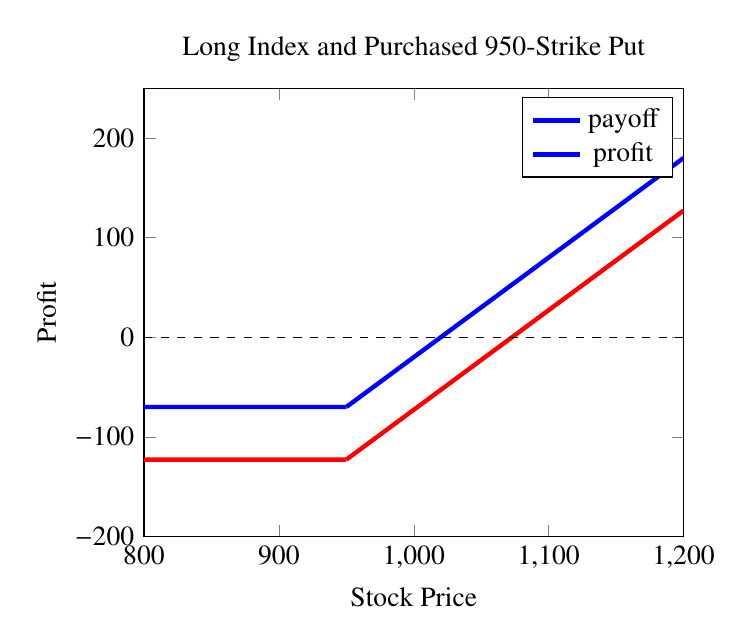
\begin{tikzpicture}
\begin{axis}[
disabledatascaling,
anchor=origin,
xmin=800,xmax=1200,
ymin=-200,ymax=250,
xlabel=Stock Price,
ylabel=Profit,
title=\text{Long Index and Purchased 950-Strike Put},
samples=50]
  \addplot[blue, ultra thick, domain=950:1200] (x,x-1020);
  \addplot[blue, ultra thick, domain=800:950] (x,x-1020 + 950-x);
  \addlegendentry{payoff};
  \addplot[red, ultra thick, domain=950:1200] (x,x-20-1000-52.813);
  \addplot[red, ultra thick, domain=800:950] (x,x-20 + 950-x-1000-52.813);
  \addlegendentry{profit};
  \addplot[black, dashed, domain=800:1200] (x,0);
\end{axis}
\end{tikzpicture}
\end{center}

Now we do the same for the \$931.37 investment and purchased 950-strike call. Again, we assume 2\% interest, so the investment grows to \$950 and the call premium grows to \$120.405. Here is the payoff and profit diagram for this position:

\begin{center}
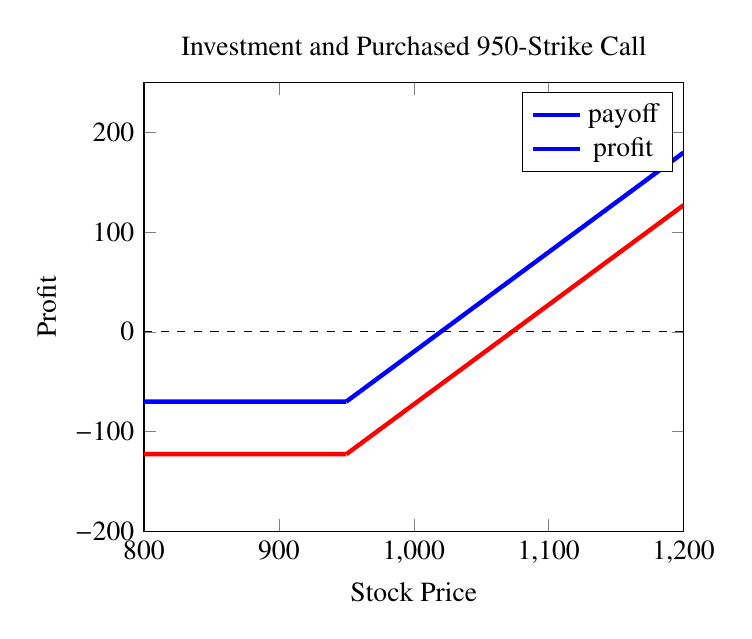
\begin{tikzpicture}
\begin{axis}[
disabledatascaling,
anchor=origin,
xmin=800,xmax=1200,
ymin=-200,ymax=250,
xlabel=Stock Price,
ylabel=Profit,
title=\text{Investment and Purchased 950-Strike Call},
samples=50]
  \addplot[blue, ultra thick, domain=950:1200] (x,x-1020);
  \addplot[blue, ultra thick, domain=800:950] (x,x-1020 + 950-x);
  \addlegendentry{payoff};
  \addplot[red, ultra thick, domain=950:1200] (x,x-20-1000-52.813);
  \addplot[red, ultra thick, domain=800:950] (x,x-20 + 950-x-1000-52.813);
  \addlegendentry{profit};
  \addplot[black, dashed, domain=800:1200] (x,0);
\end{axis}
\end{tikzpicture}
\end{center}
Which we see is indeed identical.

\problem{3.4} Suppose you short the S\&R index for \$1000 and buy a 950-strike call. Construct payoff and profit diagrams for this position. Verify that you obtain the same payoff and profit diagram by borrowing \$931.37 and buying a 950-strike put.\\

First we calculate the future value of the 950-strike call premium to be \$122.813. Here are the resulting payoff and profit diagrams for shorting the \$1000 S\&R index and purchasing the 950-strike call.

\begin{center}
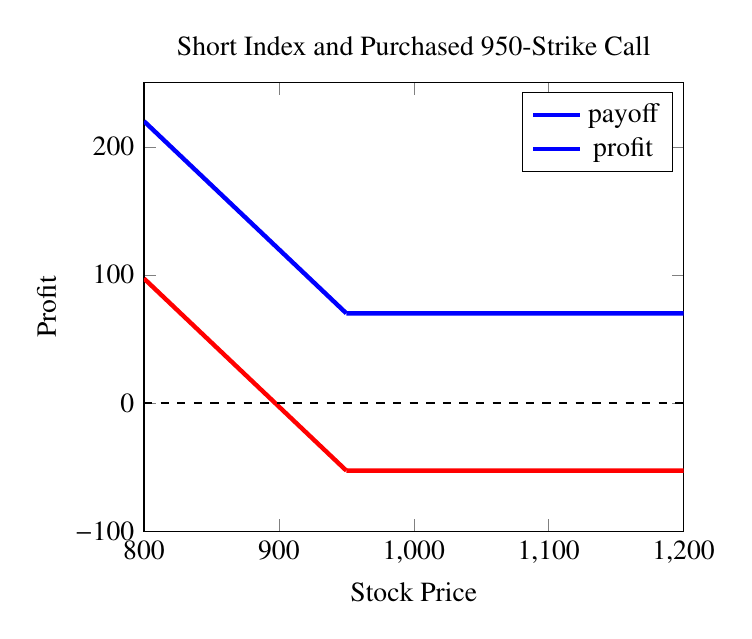
\begin{tikzpicture}
\begin{axis}[
disabledatascaling,
anchor=origin,
xmin=800,xmax=1200,
ymin=-100,ymax=250,
xlabel=Stock Price,
ylabel=Profit,
title=\text{Short Index and Purchased 950-Strike Call},
samples=50]
  \addplot[blue, ultra thick, domain=950:1200] (x,1020-x+x-950);
  \addplot[blue, ultra thick, domain=800:950] (x,1020-x);
  \addlegendentry{payoff};
  \addplot[red, ultra thick, domain=950:1200] (x,1020-x+x-950-122.813);
  \addplot[red, ultra thick, domain=800:950] (x,1020-x-122.813);
  \addlegendentry{profit};
  \addplot[black, dashed, domain=800:1200] (x,0);
\end{axis}
\end{tikzpicture}
\end{center}

Next for the borrowing and purchased put position, we first calculate that \$950 will be owed on the loan and the future value of the put premium will be \$52.813. This gives us the following payoff and profit diagrams:

\begin{center}
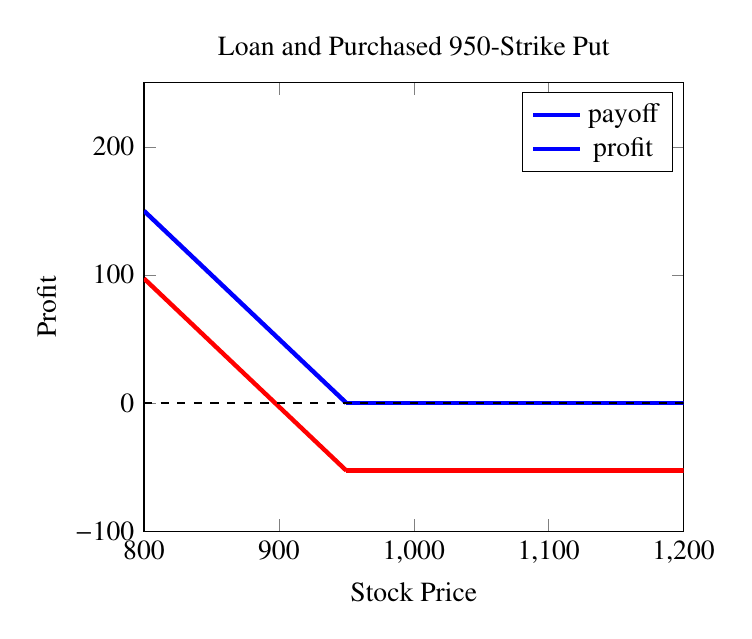
\begin{tikzpicture}
\begin{axis}[
disabledatascaling,
anchor=origin,
xmin=800,xmax=1200,
ymin=-100,ymax=250,
xlabel=Stock Price,
ylabel=Profit,
title=\text{Loan and Purchased 950-Strike Put},
samples=50]
  \addplot[blue, ultra thick, domain=950:1200] (x,0);
  \addplot[blue, ultra thick, domain=800:950] (x,950-x);
  \addlegendentry{payoff};
  \addplot[red, ultra thick, domain=950:1200] (x,0-52.813);
  \addplot[red, ultra thick, domain=800:950] (x,950-x-52.813);
  \addlegendentry{profit};
  \addplot[black, dashed, domain=800:1200] (x,0);
\end{axis}
\end{tikzpicture}
\end{center}
Although the payoff diagrams are not quite the same, the profit diagrams are identical.

\problem{3.5} Suppose you short the S\&R index for \$1000 and buy a 1050-strike call. Construct payoff and profit diagrams for this position. Verify that you obtain the same payoff and profit diagrams by borrowing \$1029.41 and buying a 1050-strike put.\\

For the short index and purchased call aggregate position, we first calculate the future premium of the call is \$73.256. Below are the payoff and profit diagrams for this position.

\begin{center}
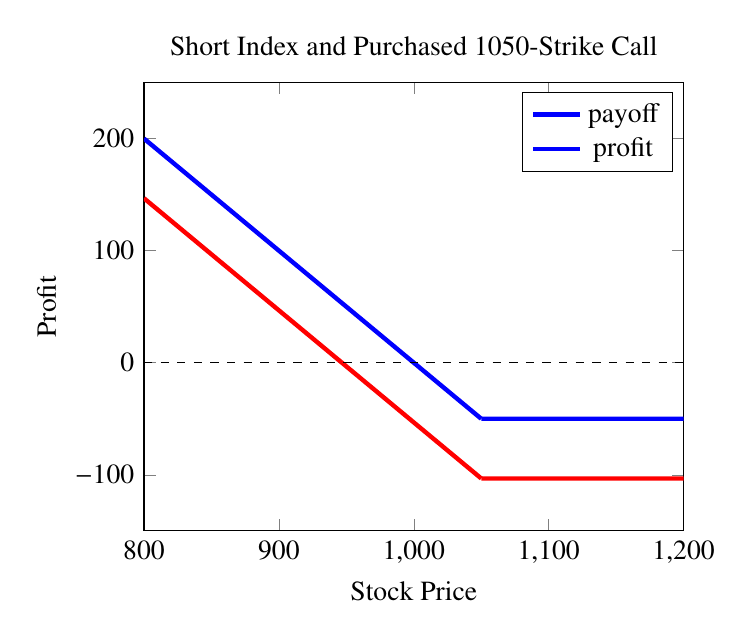
\begin{tikzpicture}
\begin{axis}[
disabledatascaling,
anchor=origin,
xmin=800,xmax=1200,
ymin=-150,ymax=250,
xlabel=Stock Price,
ylabel=Profit,
title=\text{Short Index and Purchased 1050-Strike Call},
samples=50]
  \addplot[blue, ultra thick, domain=1050:1200] (x,1000-x+x-1050);
  \addplot[blue, ultra thick, domain=800:1050] (x,1000-x);
  \addlegendentry{payoff};
  \addplot[red, ultra thick, domain=1050:1200] (x,1020-x+x-1050-73.256);
  \addplot[red, ultra thick, domain=800:1050] (x,1020-x-73.256);
  \addlegendentry{profit};
  \addplot[black, dashed, domain=800:1200] (x,0);
\end{axis}
\end{tikzpicture}
\end{center}

For the loan and purchased put position, we first calculate that \$1050 will be owed on the loan, and \$103.238 for the future value of the put premium. The payoff and profit diagrams for this position are below.

\begin{center}
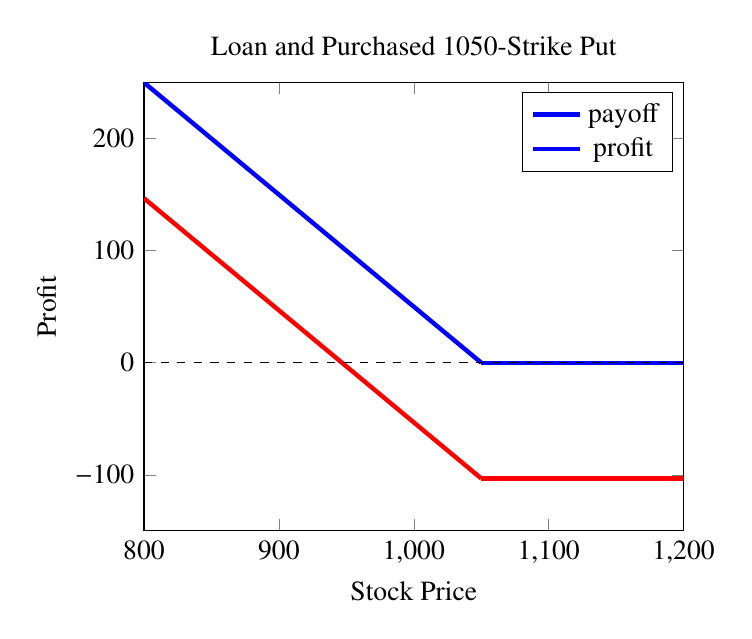
\begin{tikzpicture}
\begin{axis}[
disabledatascaling,
anchor=origin,
xmin=800,xmax=1200,
ymin=-150,ymax=250,
xlabel=Stock Price,
ylabel=Profit,
title=\text{Loan and Purchased 1050-Strike Put},
samples=50]
  \addplot[blue, ultra thick, domain=1050:1200] (x,0);
  \addplot[blue, ultra thick, domain=800:1050] (x,1050-x);
  \addlegendentry{payoff};
  \addplot[red, ultra thick, domain=1050:1200] (x,0-103.238);
  \addplot[red, ultra thick, domain=800:1050] (x,1050-x-103.238);
  \addlegendentry{profit};
  \addplot[black, dashed, domain=800:1200] (x,0);
\end{axis}
\end{tikzpicture}
\end{center}
As in the previous problem, although the payoff diagrams are not identical, the profit diagrams are.

\problem{3.6} Verify that you earn the same profit and payoff by (a) buying the S\&R index for \$1000 and (b) buying a 950-strike S\&R call, selling a 950-strike S\&R put, and lending \$931.37.\\

Let's call $x$ the value of the S\&R index. From (a) we receive a payoff of $P_a(x) = x$. From (b) we receive a payoff of $\max(0,x-950)$ from the purchased call, $\min(0,x-950)$ from the written put, and \$950 from the loan, for a total of 
\[
P_b(x) = \max(0,x-950) + \min(0,x-950) + 950 = x,
\]
so these two positions have the same payoff. 

To verify that they have the same profit, we must demonstrate that they have the same upfront cost. The cost for purchasing the S\&R index is \$1000, or \$1020 in future value. Meanwhile the cost for (b) includes the cost of \$120.405 to purchase the call, the revenue of \$51.777 for writing the put, and the cost of \$931.37 for the loan, for a total of \$1000 with a future value of \$1020. Therefore, both positions return the same profit.\\

This can also be verified using put-call parity. We let $K = 950$ be the strike price, and $T = 0.5$ the expiration time in years. Then put-call parity says that
\begin{align*}
\Call(950,0.5) - \Put(950,0.5) &= \PV(F_{0,0.5} - 950)\\
\Call(950,0.5) - \Put(950,0.5) + \PV(950) &= \PV(F_{0,0.5}).
\end{align*}

\problem{3.7} Verify that you can earn the same profit and payoff by (a) shorting the S\&R index for \$1000 and (b) selling a 1050-strike S\&R call, buying a 1050-strike put, and borrowing \$1029.41.\\

Let's call $x$ the value of the S\&R index. From (a) we receive a payoff of $P_a(x) = -x$. From (b) we receive a payoff of $\min(0,1050-x)$ from the call, $\max(0,1050-x)$ from the put, and -\$1050 from the loan, for a total of
\[
P_b(x) = \min(0,1050-x) + \max(0,1050-x) - 1050 = -x,
\]
so these two investments have the same payoff.

Let us also consider the costs of these investments. (a) has an upfront revenue of \$1000, or \$1020 in future value. (b) has an upfront cost of \$101.167 for the put, an upfront revenue of 51.873 for the call, and an upfront revenue of \$1029.41 from the loan, for a total of \$1000, or \$1020 in future value. As both investments have the same payoff and cost, they also have the same profit.\\

This can also be verified using put-call parity. We let $K = 1050$ be the strike price, and $T = 0.5$ the expiration time in years. Then put-call parity says that
\begin{align*}
\Call(1050,0.5) - \Put(1050,0.5) &= \PV(F_{0,0.5} - 1050)\\
\Put(1050,0.5) - \Call(1050,0.5) - \PV(1050) &= -\PV(F_{0,0.5}).
\end{align*}

\problem{3.8} Suppose the premium on a 6-month S\&R call is \$109.20 and the premium on a put with the same strike price is \$60.18. What is the strike price?\\

Let $K$ be the strike price, and $T = 0.5$ the expiration time measured in years. Then according to put call parity, we have
\begin{align*}
\Call(K,0.5) - \Put(K,0.5) &= \PV(F_{0,0.5} - K)\\
\$109.20 - \$60.18 &= \$1000 - \frac{K}{1.02}\\
\frac{K}{1.02} &= \$950.98\\
K &= \$967.00,
\end{align*}
so we see that the strike price must have been \$967.

\problem{3.9} Construct payoff and profit diagrams for the purchase of a 950-strike S\&R call and sale of a 1000-strike S\&R call. Verify that you obtain exactly the same \emph{profit} diagram for the purchase of a 950-strike S\&R put and sale of a 1000-strike S\&R put. What is the difference in the payoff diagrams for the call and put spreads? Why is there a difference?\\

First we analyze the first position. Suppose that the price of the index in 6 months is $x$. The payoff for a purchased 950-strike call is $\max(0,x-950)$, while the payoff for a written 1000-strike call is $\min(0,1000-x)$. The purchased 950-strike call costs a premium of \$122.813 in future value while the written 1000-strike call pays a premium of \$95.685 in future value. Thus we arrive at the payoff and profit diagrams below for this aggregate position.

\begin{center}
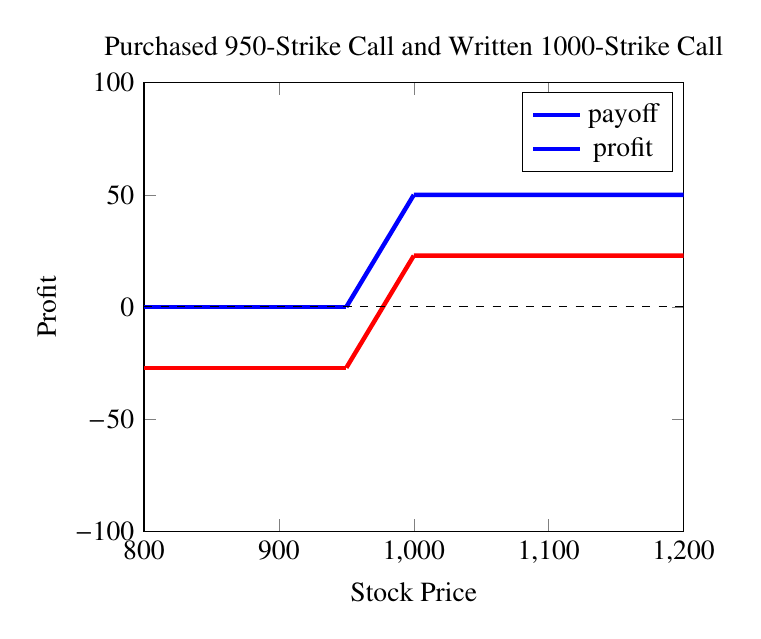
\begin{tikzpicture}
\begin{axis}[
disabledatascaling,
anchor=origin,
xmin=800,xmax=1200,
ymin=-100,ymax=100, 
xlabel=Stock Price,
ylabel=Profit,
title=\text{Purchased 950-Strike Call and Written 1000-Strike Call},
samples=50]
  \addplot[blue, ultra thick, domain=800:950] (x,0);
  \addplot[blue, ultra thick, domain=950:1000] (x,x-950);
  \addplot[blue, ultra thick, domain=1000:1200] (x,x-950+1000-x);
  \addlegendentry{payoff};
  \addplot[red, ultra thick, domain=800:950] (x,95.685 - 122.813);
  \addplot[red, ultra thick, domain=950:1000] (x,x - 950 + 95.685 - 122.813);
  \addplot[red, ultra thick, domain=1000:1200] (x,x-950 + 1000 - x+ 95.685 - 122.813);
  \addlegendentry{profit};
  \addplot[black, dashed, domain=800:1200] (x,0);
\end{axis}
\end{tikzpicture}
\end{center}

Next we analyze the second position. Suppose that the price of the index in 6 months is $x$. The payoff for a purchased 950-strike put is $\max(950-x,0)$ while the payoff for a written 1000-strike put is $\min(0,x-1000)$. The purchased 950-strike put costs \$52.813 in future value while the written 1000-strike put pays \$75.685 in future value. Thus we arrive at the payoff and profit diagrams below for this aggregate position.

\begin{center}
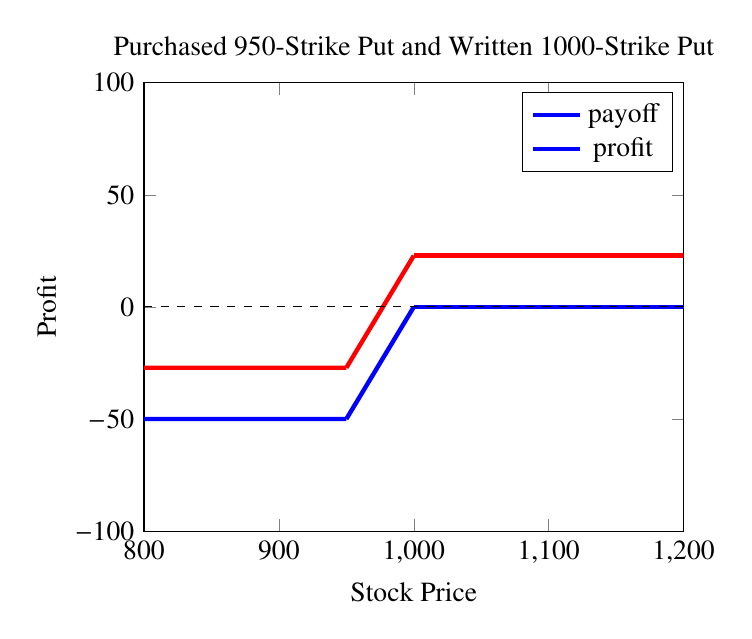
\begin{tikzpicture}
\begin{axis}[
disabledatascaling,
anchor=origin,
xmin=800,xmax=1200,
ymin=-100,ymax=100, 
xlabel=Stock Price,
ylabel=Profit,
title=\text{Purchased 950-Strike Put and Written 1000-Strike Put},
samples=50]
  \addplot[blue, ultra thick, domain=800:950] (x,950-x + x-1000);
  \addplot[blue, ultra thick, domain=950:1000] (x,x-1000);
  \addplot[blue, ultra thick, domain=1000:1200] (x,0);
  \addlegendentry{payoff};
  \addplot[red, ultra thick, domain=800:950] (x,950-x + x-1000 + 75.685 - 52.813);
  \addplot[red, ultra thick, domain=950:1000] (x,x-1000+75.685 - 52.813);
  \addplot[red, ultra thick, domain=1000:1200] (x,75.685 - 52.813);
  \addlegendentry{profit};
  \addplot[black, dashed, domain=800:1200] (x,0);
\end{axis}
\end{tikzpicture}
\end{center}

We can see that although the profit diagrams are equal, the payoff diagrams are not. The payoff diagram for the second option is exactly \$50 lower than the payoff diagram for the first option. This is because the first position has a positive upfront cost while the second position has a negative upfront cost. The higher upfront cost of the first position is exactly offset by the higher payoff, giving the same profit diagram for both.

\problem{3.10} Construct payoff and profit diagrams for the purchase of a 1050-strike S\&R call and sale of a 950-strike S\&R call. Verify that you obtain exactly the same \emph{profit} diagram for the purchase of a 1050-strike S\&R put and sale of a 950-strike S\&R put. What is the difference in the initial cost of these positions?

First we analyze the first position. Suppose that the price of the index in 6 months is $x$. The payoff for the purchase of a 1050-strike call is $\max(0,x-1050)$ and the payoff for writing a 950-strike call is $\min(0,950-x)$. Purchasing the 1050-strike call costs \$73.238 in future value while writing the 950-strike call pays \$122.813 in future value. Thus we arrive at the payoff and profit diagrams below.

\begin{center}
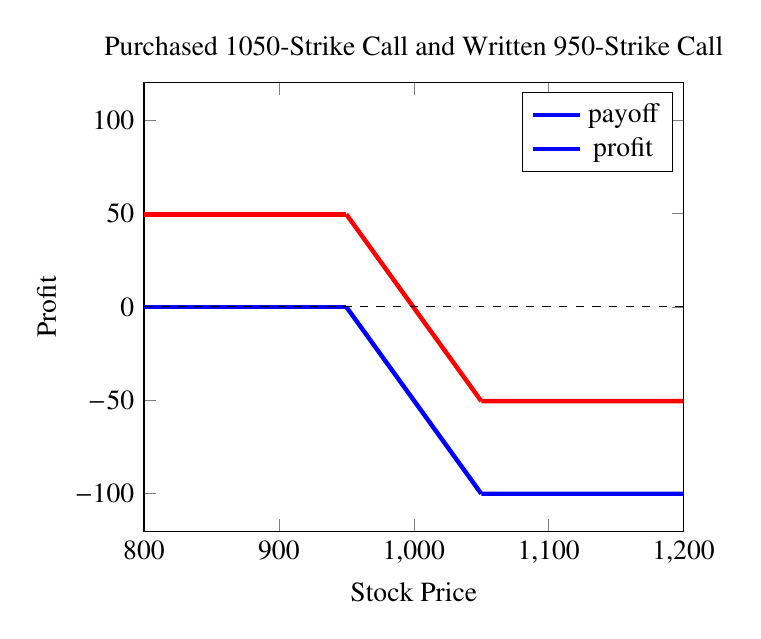
\begin{tikzpicture}
\begin{axis}[
disabledatascaling,
anchor=origin,
xmin=800,xmax=1200,
ymin=-120,ymax=120, 
xlabel=Stock Price,
ylabel=Profit,
title=\text{Purchased 1050-Strike Call and Written 950-Strike Call},
samples=50]
  \addplot[blue, ultra thick, domain=800:950] (x,0);
  \addplot[blue, ultra thick, domain=950:1050] (x,950-x);
  \addplot[blue, ultra thick, domain=1050:1200] (x,950-x+x-1050);
  \addlegendentry{payoff};
  \addplot[red, ultra thick, domain=800:950] (x,0 + 122.813 - 73.238);
  \addplot[red, ultra thick, domain=950:1050] (x,950-x + 122.813 - 73.238);
  \addplot[red, ultra thick, domain=1050:1200] (x,950-x+x-1050 + 122.813 - 73.238);
  \addlegendentry{profit};
  \addplot[black, dashed, domain=800:1200] (x,0);
\end{axis}
\end{tikzpicture}
\end{center}

Next we analyze the second position. Suppose that the price of the index in 6 months is $x$. The payoff for the purchase of a 1050-strike put is $\max(0,1050-x)$ and the payoff for writing a 950-strike put is $\min(0,x-950)$. Purchasing the 1050-strike put costs \$103.238 in future value, while writing the 950-strike put pays \$52.813 in future value. Thus we arrive at the payoff and profit diagrams below.

\begin{center}
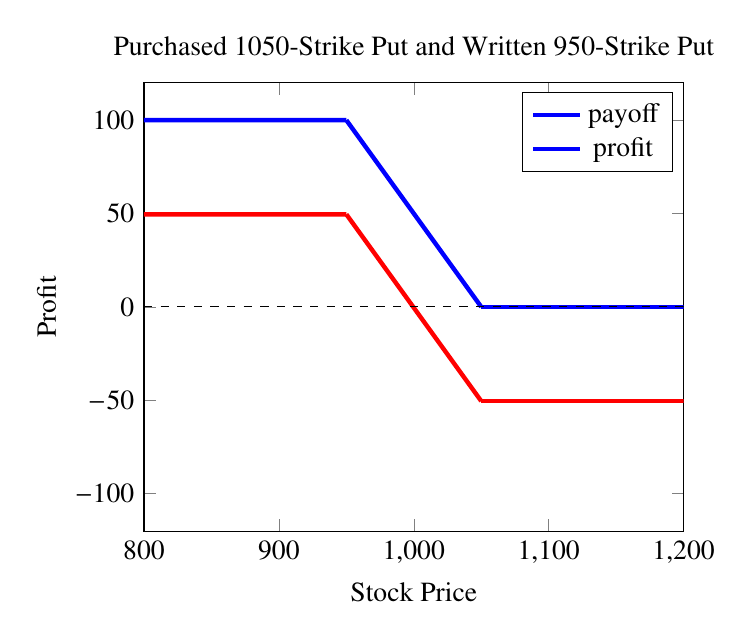
\begin{tikzpicture}
\begin{axis}[
disabledatascaling,
anchor=origin,
xmin=800,xmax=1200,
ymin=-120,ymax=120, 
xlabel=Stock Price,
ylabel=Profit,
title=\text{Purchased 1050-Strike Put and Written 950-Strike Put},
samples=50]
  \addplot[blue, ultra thick, domain=800:950] (x,1050-x+x-950);
  \addplot[blue, ultra thick, domain=950:1050] (x,1050-x);
  \addplot[blue, ultra thick, domain=1050:1200] (x,0);
  \addlegendentry{payoff};
  \addplot[red, ultra thick, domain=800:950] (x,1050-x+x-950+52.813-103.238);
  \addplot[red, ultra thick, domain=950:1050] (x,1050-x+52.813-103.238);
  \addplot[red, ultra thick, domain=1050:1200] (x,0+52.813-103.238);
  \addlegendentry{profit};
  \addplot[black, dashed, domain=800:1200] (x,0);
\end{axis}
\end{tikzpicture}
\end{center}

As in the previous problem we see that the profit diagrams are identical even though the payoff diagrams are not. This is because the first position has a negative upfront cost while the second position has a positive upfront cost. However, the higher upfront cost of the second position is exactly balanced by increased payoffs.

\problem{3.11} Suppose you invest in the S\&R index for \$1000, buy a 950-strike put, and sell a 1050-strike call. Draw a profit diagram for this position. What is the net option premium? If you wanted to construct a zero-cost collar keeping the put strike equal to \$950, in what direction would you have to change the call strike?\\

Suppose that the price of the index in 6 months is $x$. The payoff from the long position on the index is then also $x$, the payoff for a purchased 950-strike put is $\max(0,950-x)$, and the payoff for a written 1050-strike call is $\min(0,1050-x)$. The long position on the index costs \$1020 in future value, purchasing the 950-strike put costs \$52.813 in future value, and writing the 1050-strike call pays \$73.238 in future value. Thus we arrive at the payoff and profit diagrams below.

\begin{center}
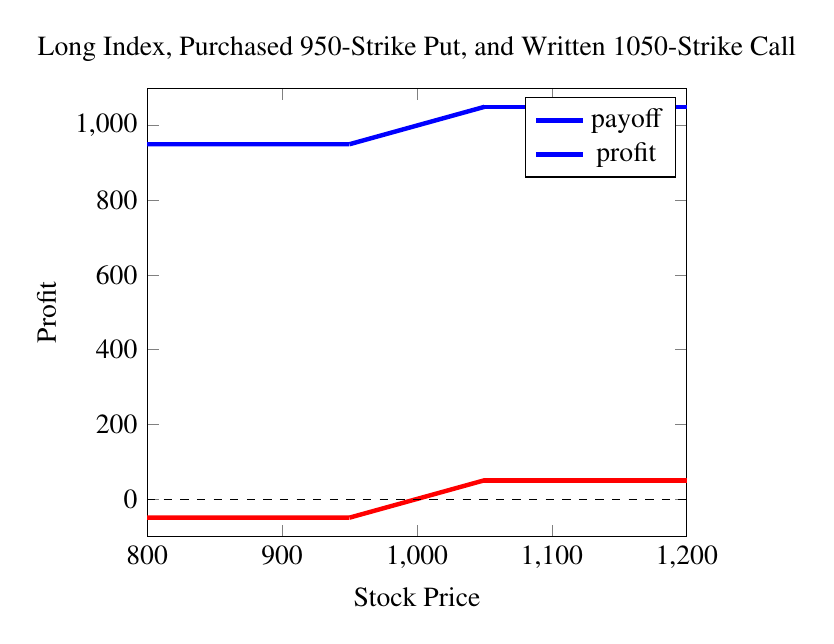
\begin{tikzpicture}
\begin{axis}[
disabledatascaling,
anchor=origin,
xmin=800,xmax=1200,
ymin=-100,ymax=1100, 
xlabel=Stock Price,
ylabel=Profit,
title=\text{Long Index, Purchased 950-Strike Put, and Written 1050-Strike Call},
samples=50]
  \addplot[blue, ultra thick, domain=800:950] (x,x+950-x);
  \addplot[blue, ultra thick, domain=950:1050] (x,x);
  \addplot[blue, ultra thick, domain=1050:1200] (x,x+1050-x);
  \addlegendentry{payoff};
  \addplot[red, ultra thick, domain=800:950] (x,x+950-x+73.238-52.813-1020);
  \addplot[red, ultra thick, domain=950:1050] (x,x+73.238-52.813-1020);
  \addplot[red, ultra thick, domain=1050:1200] (x,x+1050-x+73.238-52.813-1020);
  \addlegendentry{profit};
  \addplot[black, dashed, domain=800:1200] (x,0);
\end{axis}
\end{tikzpicture}
\end{center}
The net option premium for this position is -\$20.425 in future value. To make a zero-cost collar keeping the put strike equal to 950, you would need to increase the strike of the call as strike value and premium are inversely related for calls.

\problem{3.12} Suppose you invest in the S\&R index for \$1000, buy a 950-strike put, and sell a 1107-strike call. Draw a profit diagram for this position. How close is this to a zero-cost collar? \\

Suppose that the price of the index in 6 months is $x$. The payoff from the long position on the index is then also $x$, the payoff from the purchased 950-strike put is $\max(0,950-x)$, and the payoff from the written 1107-strike put is $\min(0,1107-x)$. The long position on the index costs \$1020 in future value, purchasing the 950-strike put costs \$52.813 in future value, and writing the 1107-strike call costs \$52.910 in future value. Thus we arrive at the payoff and profit diagrams below.

\begin{center}
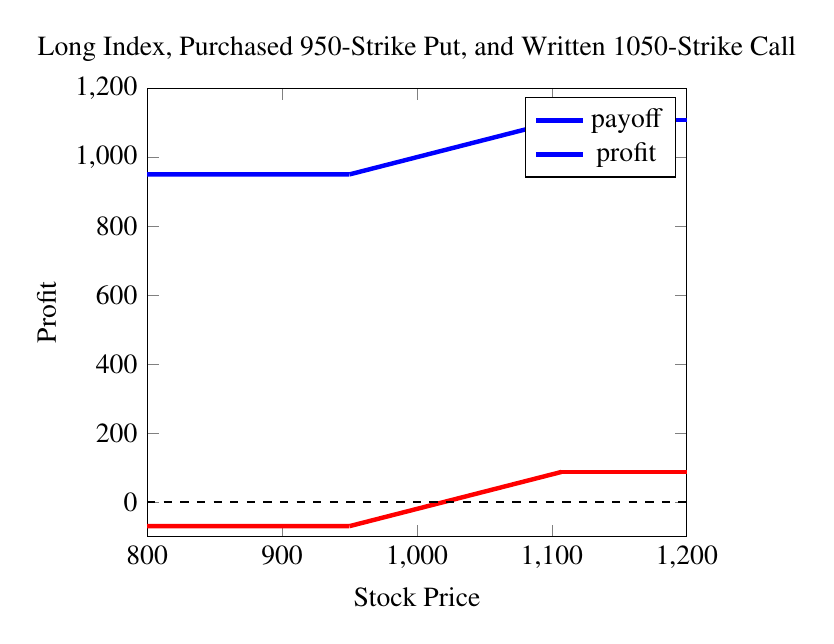
\begin{tikzpicture}
\begin{axis}[
disabledatascaling,
anchor=origin,
xmin=800,xmax=1200,
ymin=-100,ymax=1200, 
xlabel=Stock Price,
ylabel=Profit,
title=\text{Long Index, Purchased 950-Strike Put, and Written 1050-Strike Call},
samples=50]
  \addplot[blue, ultra thick, domain=800:950] (x,x+950-x);
  \addplot[blue, ultra thick, domain=950:1107] (x,x);
  \addplot[blue, ultra thick, domain=1107:1200] (x,x+1107-x);
  \addlegendentry{payoff};
  \addplot[red, ultra thick, domain=800:950] (x,x+950-x+52.910-52.813-1020);
  \addplot[red, ultra thick, domain=950:1107] (x,x+52.910-52.813-1020);
  \addplot[red, ultra thick, domain=1107:1200] (x,x+1107-x+52.910-52.813-1020);
  \addlegendentry{profit};
  \addplot[black, dashed, domain=800:1200] (x,0);
\end{axis}
\end{tikzpicture}
\end{center}
This is very close to being a zero-cost collar the net option premium is -\$0.097 in future value.

\problem{3.13} Draw profit diagrams for the following positions:
\begin{enumerate}[(a)]
\item 1050-strike S\&R straddle.\\

\begin{center}
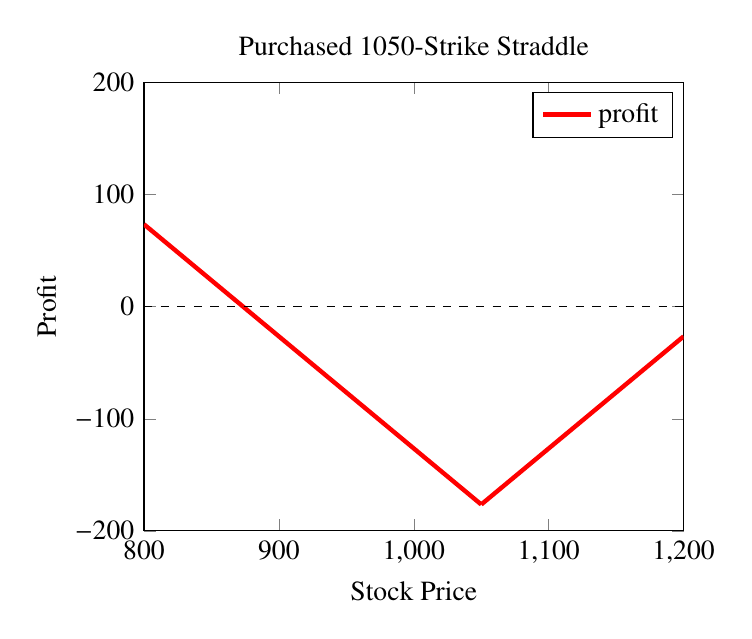
\begin{tikzpicture}
\begin{axis}[
disabledatascaling,
anchor=origin,
xmin=800,xmax=1200,
ymin=-200,ymax=200, 
xlabel=Stock Price,
ylabel=Profit,
title=\text{Purchased 1050-Strike Straddle},
samples=50]
  \addplot[red, ultra thick, domain=800:1050] (x,1050-x-176.476);
  \addplot[red, ultra thick, domain=1050:1200] (x,x-1050-176.476);
  \addlegendentry{profit};
  \addplot[black, dashed, domain=800:1200] (x,0);
\end{axis}
\end{tikzpicture}
\end{center}

\item Written 950-strike S\&R straddle.\\

\begin{center}
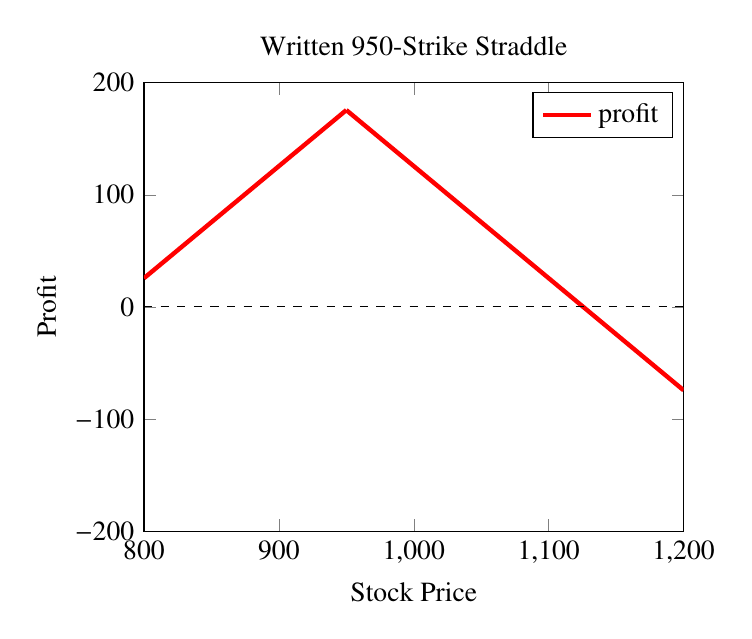
\begin{tikzpicture}
\begin{axis}[
disabledatascaling,
anchor=origin,
xmin=800,xmax=1200,
ymin=-200,ymax=200, 
xlabel=Stock Price,
ylabel=Profit,
title=\text{Written 950-Strike Straddle},
samples=50]
  \addplot[red, ultra thick, domain=800:950] (x,x-950+175.626);
  \addplot[red, ultra thick, domain=950:1200] (x,950-x+175.626);
  \addlegendentry{profit};
  \addplot[black, dashed, domain=800:1200] (x,0);
\end{axis}
\end{tikzpicture}
\end{center}

\item Simultaneous purchase of a 1050-strike straddle and sale of a 950-strike S\&R straddle.\\

\begin{center}
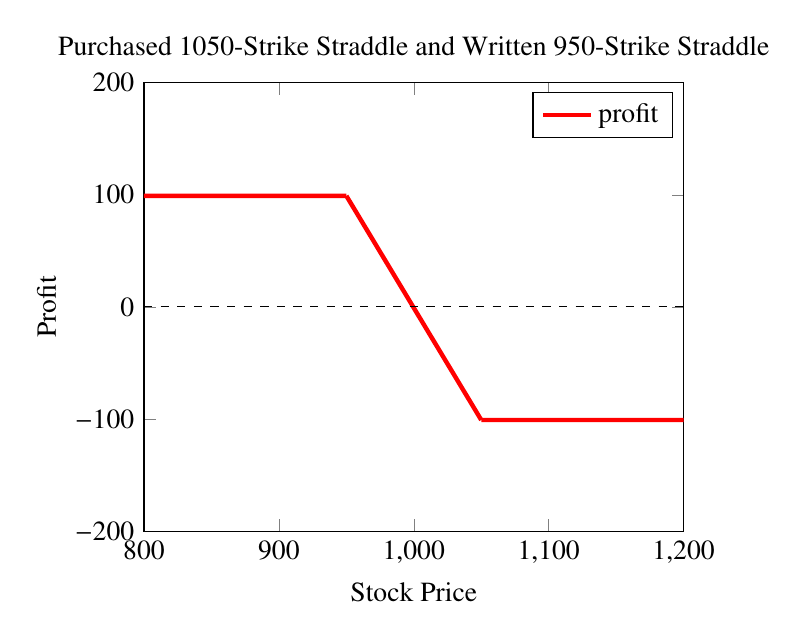
\begin{tikzpicture}
\begin{axis}[
disabledatascaling,
anchor=origin,
xmin=800,xmax=1200,
ymin=-200,ymax=200, 
xlabel=Stock Price,
ylabel=Profit,
title=\text{Purchased 1050-Strike Straddle and Written 950-Strike Straddle},
samples=50]
  \addplot[red, ultra thick, domain=800:950] (x,x-950+175.626+1050-x-176.476);
  \addplot[red, ultra thick, domain=950:1050] (x,950-x+175.626+1050-x-176.476);
  \addplot[red, ultra thick, domain=1050:1200] (x,950-x+175.626+x-1050-176.476);
  \addlegendentry{profit};
  \addplot[black, dashed, domain=800:1200] (x,0);
\end{axis}
\end{tikzpicture}
\end{center}
\end{enumerate}

\problem{3.14} Suppose you buy a 950-strike S\&R call, sell a 1000-strike S\&R call, sell a 950-strike S\&R put, and buy a 1000-strike S\&R put.
\begin{enumerate}[(a)]
\item Verify that there is no S\&R price risk in this transaction.\\

Let $x$ be the price of the index in 6 months. We can show that this position has no price risk by computing the payoff and showing that it does not depend on $x$. The payoff for purchasing a 950-strike call is $\max(0,x-950)$, the payoff for writing a 1000-strike call is $\min(0,1000-x)$, the payoff for writing a 950-strike put is $\min(0,x-950)$, and the payoff for purchasing a 1000-strike put is $\max(0,1000-x)$. Adding these together, we see that
\begin{align*}
\text{Payoff} &= \max(0,x-950) + \min(0,1000-x) + \min(0,x-950) + \max(0,1000-x)\\
&= \left[\max(0,x-950) + \min(0,x-950)\right] + \left[\max(0,1000-x) + \min(1000-x)\right]\\
&= x-950 + 1000-x\\
&= 50,
\end{align*}
using the following property of minimums and maximums: $\max(a,b) + \min(a,b) = a + b$.

\item What is the initial cost of the position?\\

Purchasing the 950-strike call costs \$120.405, writing the 1000-strike call pays \$93.809, writing the 950-strike put pays \$51.777, and purchasing the 1000-strike put costs \$74.201. So in total the position costs \$49.02.

\item What is the value of the position after 6 months?\\

The value of the position after 6 months is \$50, we can see this from our payoff computation in part (a).

\item Verify that the implicit interest rate in these cash flows is 2\% over 6 months.\\

Since $1.02 \cdot \$49.02 = \$50$, we can verify that the implicit interest rate in these cash flows is 2\%.
\end{enumerate}

\problem{3.15} Compute profit diagrams for the following ratio spreads:
\begin{enumerate}[(a)]
\item Buy 950-strike call, sell two 1050-strike calls.\\

\begin{center}
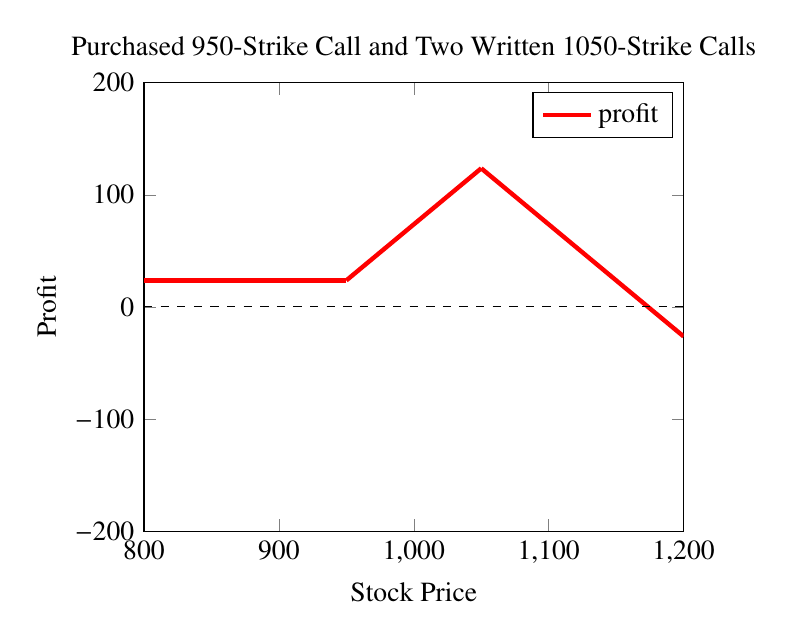
\begin{tikzpicture}
\begin{axis}[
disabledatascaling,
anchor=origin,
xmin=800,xmax=1200,
ymin=-200,ymax=200, 
xlabel=Stock Price,
ylabel=Profit,
title=\text{Purchased 950-Strike Call and Two Written 1050-Strike Calls},
samples=50]
  \addplot[red, ultra thick, domain=800:950] (x,0+23.66298);
  \addplot[red, ultra thick, domain=950:1050] (x,x-950+23.66298);
  \addplot[red, ultra thick, domain=1050:1200] (x,x-950-2*x+2100+23.66298);
  \addlegendentry{profit};
  \addplot[black, dashed, domain=800:1200] (x,0);
\end{axis}
\end{tikzpicture}
\end{center}

\item Buy two 950-strike calls, sell three 1050-strike calls.\\

\begin{center}
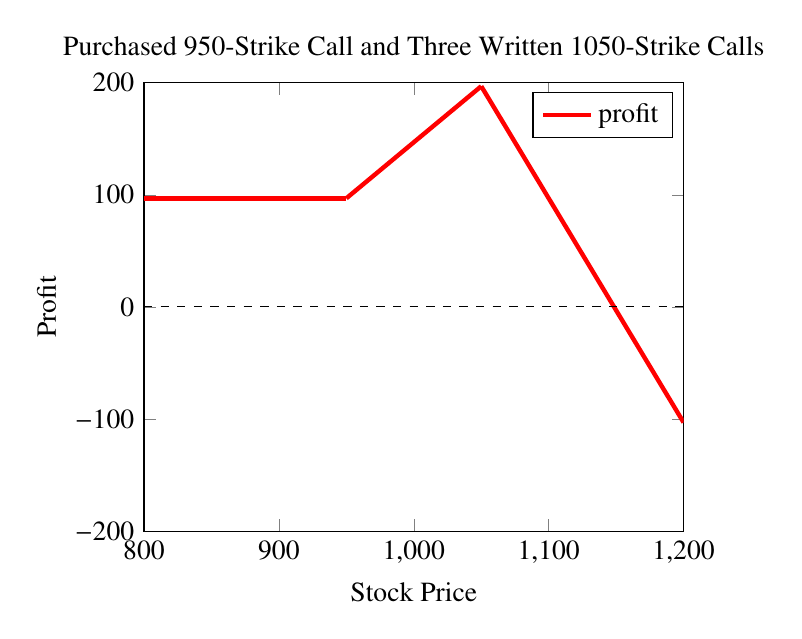
\begin{tikzpicture}
\begin{axis}[
disabledatascaling,
anchor=origin,
xmin=800,xmax=1200,
ymin=-200,ymax=200, 
xlabel=Stock Price,
ylabel=Profit,
title=\text{Purchased 950-Strike Call and Three Written 1050-Strike Calls},
samples=50]
  \addplot[red, ultra thick, domain=800:950] (x,0+96.910);
  \addplot[red, ultra thick, domain=950:1050] (x,x-950+96.910);
  \addplot[red, ultra thick, domain=1050:1200] (x,x-950-3*x+3150+96.910);
  \addlegendentry{profit};
  \addplot[black, dashed, domain=800:1200] (x,0);
\end{axis}
\end{tikzpicture}
\end{center}

\item Consider buying $n$ 950-strike calls and selling $m$ 1050-strike calls so that the premium of the position is zero. Considering your analysis in (a) and (b), what can you say about $n/m$? What exact ratio gives you a zero premium?\\

The zero premium would need to satisfy $120.405n - 71.802m = 0$, which can be rearranged to:
\begin{align*}
120.405n - 71.802m &= 0\\
120.405n &= 71.802m \\
\frac{n}{m} &= \frac{71.802}{120.405} = 0.5963,
\end{align*}
so $n/m = 0.5963$ is necessary to achieve a premium of zero.

\end{enumerate}

\problem{3.16} In the previous problem we saw that a ratio spread can have zero initial premium. Can a bull spread or bear spread have zero initial premium? A butterfly spread? Why or why not?\\

A bull spread spread cannot have be constructed for zero initial premium. This is because a bull spread involves buying a call and selling a call with a different strike value. This means that the premiums coming in and premiums going out cannot be the same unless the strike prices are identical, which would be the same as having no position. A bear spread cannot have zero premium for the same reason.

A zero premium butterfly spread is also not possible. Suppose you write a straddle with expiration time $T$ around a peak price of $K$. Then you would need to find $L$ such that
\[
\Call(K+L,T) + \Put(K-L,T) = \Straddle(K,T)
\]
to achieve a zero premium butterfly spread. This equation is equal when $L = 0$, as writing the butterfly spread involves writing a put and call with equal strike price. As $\Call(K + L,T)$ and $\Put(K-L,T)$ are both decreasing in $L$, there are no other values of $L$ that make the two sides of the equation equal. Therefore, a zero premium butterfly spread is only possible when the position is equivalent to having no position.

\problem{3.17} Construct an asymmetric butterfly spread using the 950-, 1020-, and 1050-strike options. How many of each option do you hold? Draw a profit diagram for the position.\\

Since 1020 is 70\% of the way between 950 and 1050, we would want to write ten 1020-strike calls, purchase three 950-strike calls, and purchase seven 1050-strike calls. This gives us the profit diagram below.

\begin{center}
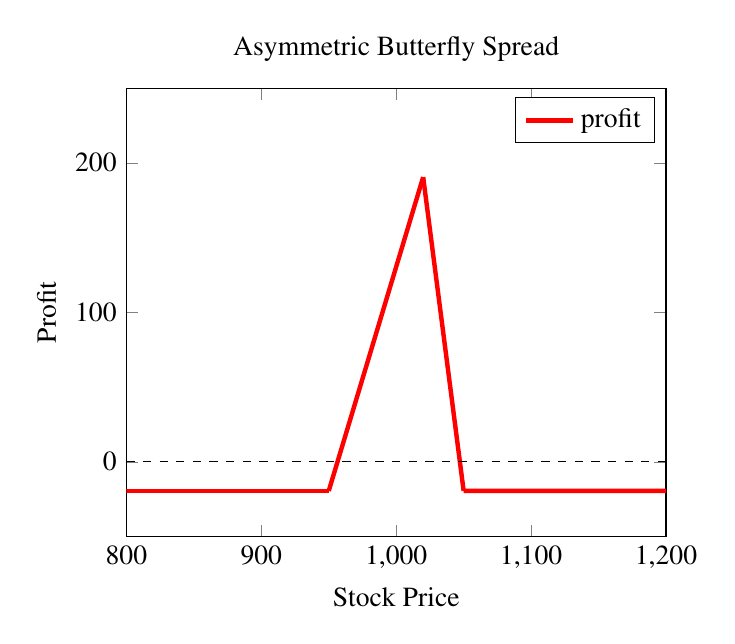
\begin{tikzpicture}
\begin{axis}[
disabledatascaling,
anchor=origin,
xmin=800,xmax=1200,
ymin=-50,ymax=250, 
xlabel=Stock Price,
ylabel=Profit,
title=\text{Asymmetric Butterfly Spread},
samples=50]
  \addplot[red, ultra thick, domain=800:950] (x,0-19.512);
  \addplot[red, ultra thick, domain=950:1020] (x,3*x-3*950-19.512);
  \addplot[red, ultra thick, domain=1020:1050] (x,3*x-3*950+10*1020-10*x-19.512);
  \addplot[red, ultra thick, domain=1050:1200] (x,3*x-3*950+10*1020-10*x+7*x-7*1050-19.512);
  \addlegendentry{profit};
  \addplot[black, dashed, domain=800:1200] (x,0);
\end{axis}
\end{tikzpicture}
\end{center}

\problem{3.18} Verify that the butterfly spread in Figure 3.14 can be duplicated by the following transactions (use the option prices in Table 3.4):
\begin{enumerate}[(a)]
\item Buy 35 call, sell two 40 calls, buy 45 call.\\

This gives us the following profit diagram:
\begin{center}
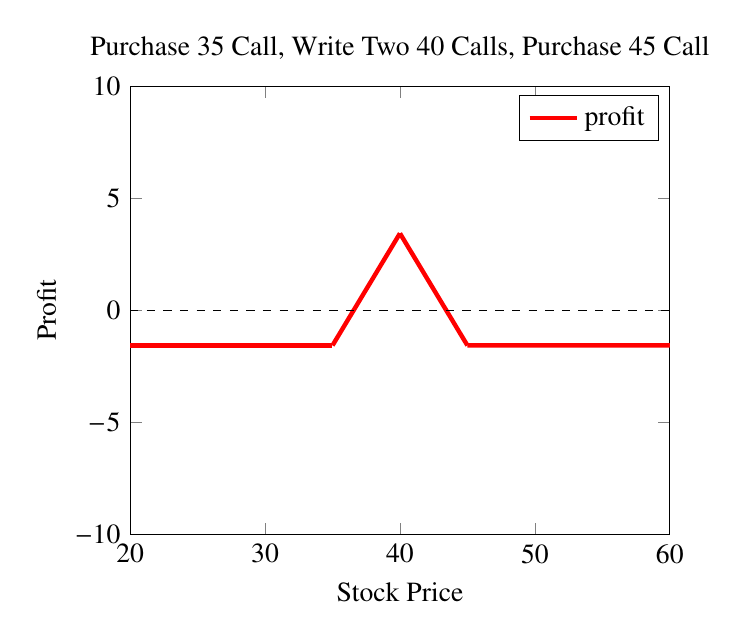
\begin{tikzpicture}
\begin{axis}[
disabledatascaling,
anchor=origin,
xmin=20,xmax=60,
ymin=-10,ymax=10, 
xlabel=Stock Price,
ylabel=Profit,
title=\text{Purchase 35 Call, Write Two 40 Calls, Purchase 45 Call},
samples=50]
  \addplot[red, ultra thick, domain=20:35] (x,0-1.57111475);
  \addplot[red, ultra thick, domain=35:40] (x,x-35-1.57111475);
  \addplot[red, ultra thick, domain=40:45] (x,x-35+2*40-2*x-1.57111475);
  \addplot[red, ultra thick, domain=45:60] (x,x-35+2*40-2*x+x-45-1.57111475);
  \addlegendentry{profit};
  \addplot[black, dashed, domain=20:60] (x,0);
\end{axis}
\end{tikzpicture}
\end{center}
We can see that this is identical to Figure 3.14.

\item Buy 35 put, sell two 40 puts, buy 45 put.\\

This gives us the following profit diagram:
\begin{center}
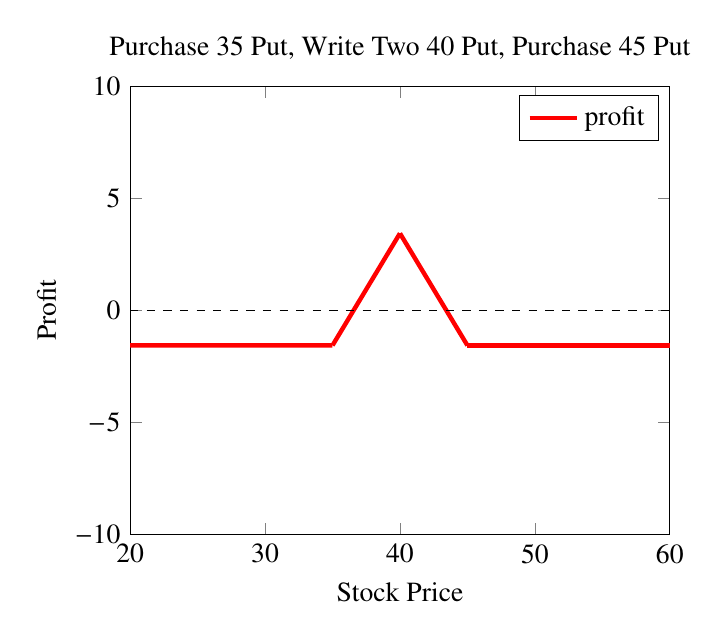
\begin{tikzpicture}
\begin{axis}[
disabledatascaling,
anchor=origin,
xmin=20,xmax=60,
ymin=-10,ymax=10, 
xlabel=Stock Price,
ylabel=Profit,
title=\text{Purchase 35 Put, Write Two 40 Put, Purchase 45 Put},
samples=50]
  \addplot[red, ultra thick, domain=20:35] (x,45-x+2*x-2*40+35-x-1.57);
  \addplot[red, ultra thick, domain=35:40] (x,45-x+2*x-2*40-1.57);
  \addplot[red, ultra thick, domain=40:45] (x,45-x-1.57);
  \addplot[red, ultra thick, domain=45:60] (x,0-1.57);
  \addlegendentry{profit};
  \addplot[black, dashed, domain=20:60] (x,0);
\end{axis}
\end{tikzpicture}
\end{center}
We can see that his is identical to Figure 3.14.

\item Buy stock, buy 35 put, sell two 40 calls, buy 45 call.\\

This gives us the following profit diagram:
\begin{center}
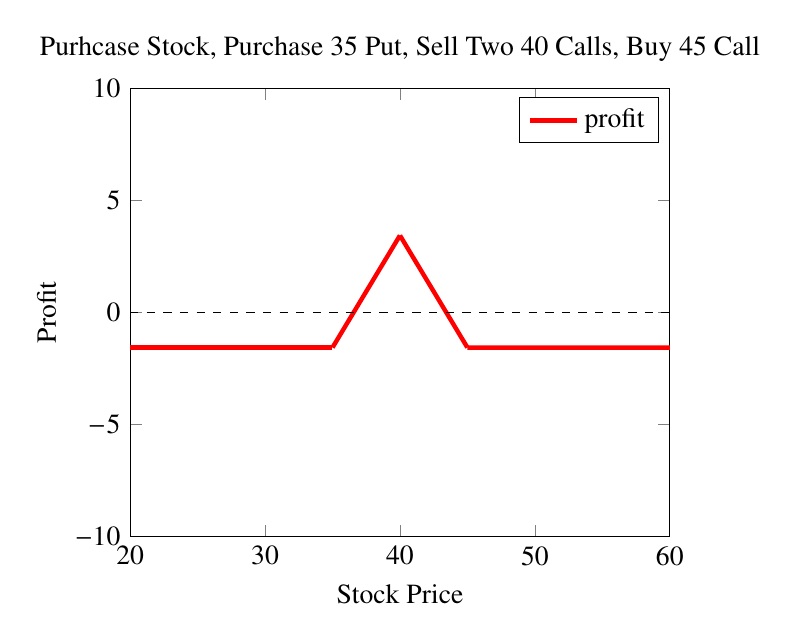
\begin{tikzpicture}
\begin{axis}[
disabledatascaling,
anchor=origin,
xmin=20,xmax=60,
ymin=-10,ymax=10, 
xlabel=Stock Price,
ylabel=Profit,
title=\text{Purhcase Stock, Purchase 35 Put, Sell Two 40 Calls, Buy 45 Call},
samples=50]
  \addplot[red, ultra thick, domain=20:35] (x,x+35-x-36.57);
  \addplot[red, ultra thick, domain=35:40] (x,x-36.57);
  \addplot[red, ultra thick, domain=40:45] (x,x+2*40-2*x-36.57);
  \addplot[red, ultra thick, domain=45:60] (x,x+2*40-2*x+x-45-36.57);
  \addlegendentry{profit};
  \addplot[black, dashed, domain=20:60] (x,0);
\end{axis}
\end{tikzpicture}
\end{center}
We can see that this is identical to Figure 3.14.
\end{enumerate}

\problem{3.19} Here is a quote from an investment website about an investment strategy using options:
\begin{quotation}
One strategy investors are applying to the XYZ options is using ``synthetic stock." A synthetic stock is created when an investor simultaneously purchases a call option and sells a put option on the same stock. The end result is that the synthetic stock has the same value, in terms of capital gain potential, as the underlying stock itself. Provided the premiums on the options are the same, they cancel each other out so the transaction fees are a wash.
\end{quotation}

Suppose, to be concrete, that the premium on the call you buy is the same as the premium on the put you sell, and both have the same strikes and times to expiration.
\begin{enumerate}[(a)]
\item What can you say about the strike price?\\

For this option to have the same value as the stock, we would need the strike price of the put and call to be equal. Otherwise there would be some portion of the profit diagram which is flat (either where the put and call are both flat or neither are flat). Since call premiums decrease with strike value and put premiums increase with strike value, the only way to accomplish this is if both strike values are the forward price.

\item What term best describes the position you have created?\\

I suppose this is a written collar with zero width and zero cost? A terser description would be a forward contract.

\item Suppose the options have a bid-ask spread. If you are creating a synthetic purchased stock and the net premium is zero \emph{inclusive of the bid-ask spread}, where will the strike price be relative to the forward price?\\

Call premiums decrease with strike price while put premiums increase with strike price. So to have a small margin for the bid-ask spread you would need the put premium to be slightly above the call premium, which would put the strike price slightly above the forward price.

\item If you create a synthetic short stock with zero premium inclusive of the bid-ask spread, where will the strike price be relative to the forward price?\\

Call premiums decrease with strike price while put premiums increase with strike price. So to have a small margin for the bid-ask spread you would need the call premium to be slightly above the put premium, which would put the strike price slightly below the forward price.

\item Do you consider the ``transaction fees" to really be ``a wash"? Why or why not?\\

It would depend on the market maker's fee structure. If the bid-ask spread for the synthetic stock is the same as the bid-ask spread for a forward contract, then they would be the same. However, if the bid-ask spread is the same for each contract whether it be forward, put, or call, then the synthetic stock is strictly worse than the forward contract. There might also be tax incentives for one position or the other.

In general the market should settle on fee structures that make these positions identical. Otherwise investors would buy one and sell the other to make a profit, which would drive down the cost of one and drive up the cost of the other until they become the same.
\end{enumerate}

\problem{3.20} Construct a spreadsheet for which you can input up to five stock prices and quantities of put and call options bought or sold at those strikes, and which will automatically construct the total expiration payoff diagram for that position. Modify the spreadsheet to permit you to choose whether to graph a payoff or profit function.\\

This spreadsheet can be found at
\begin{verbatim}
McDonald_Chapter2.xls
\end{verbatim}
In the same folder as this file.

\end{document}